\chapter{Aims}
BedSAT: Antarctica is a modelling approach that combines satellite observations of the ice surface, airborne radar surveys of the bed, and numerical ice flow modelling. It is physically informed by observed bed morphometry statistics which feed into synthetic bedrock generation for ISSM ice-sheet models. With BedSAT we aim to use machine learning to model bed-to-surface transfer from physics-based simulations over these synthetic beds, and to invert the transfer process, so that observed surface expression from real satellite data can be mapped back to bed topography. The goal of this project is to improve the resolution and accuracy of Antarctic bed topography.

\section{Project Deliverables}
\begin{itemize}
    \item\textbf{Paper 1 — ODSA}: Develop a physically informed spectral analysis framework for quantifying Antarctic subglacial landscape characteristics and classifying bed morphology into archetypes for ice sheet modelling;
    \item\textbf{Paper 2 — Bedrock factory}: Design a synthetic bed topography generator for Antarctic landscapes that takes morphometric statistics from ODSA as inputs and produces bed realisations at ice sheet model resolution.
    \item\textbf{Paper 1 — BedSAT}: Develop a modelling approach that combines satellite
    remote sensing, airborne radar and numerical ice flow modelling to improve the
    resolution and accuracy of Antarctic bed topography.
\end{itemize}

\section{Timeline}
\begin{figure}
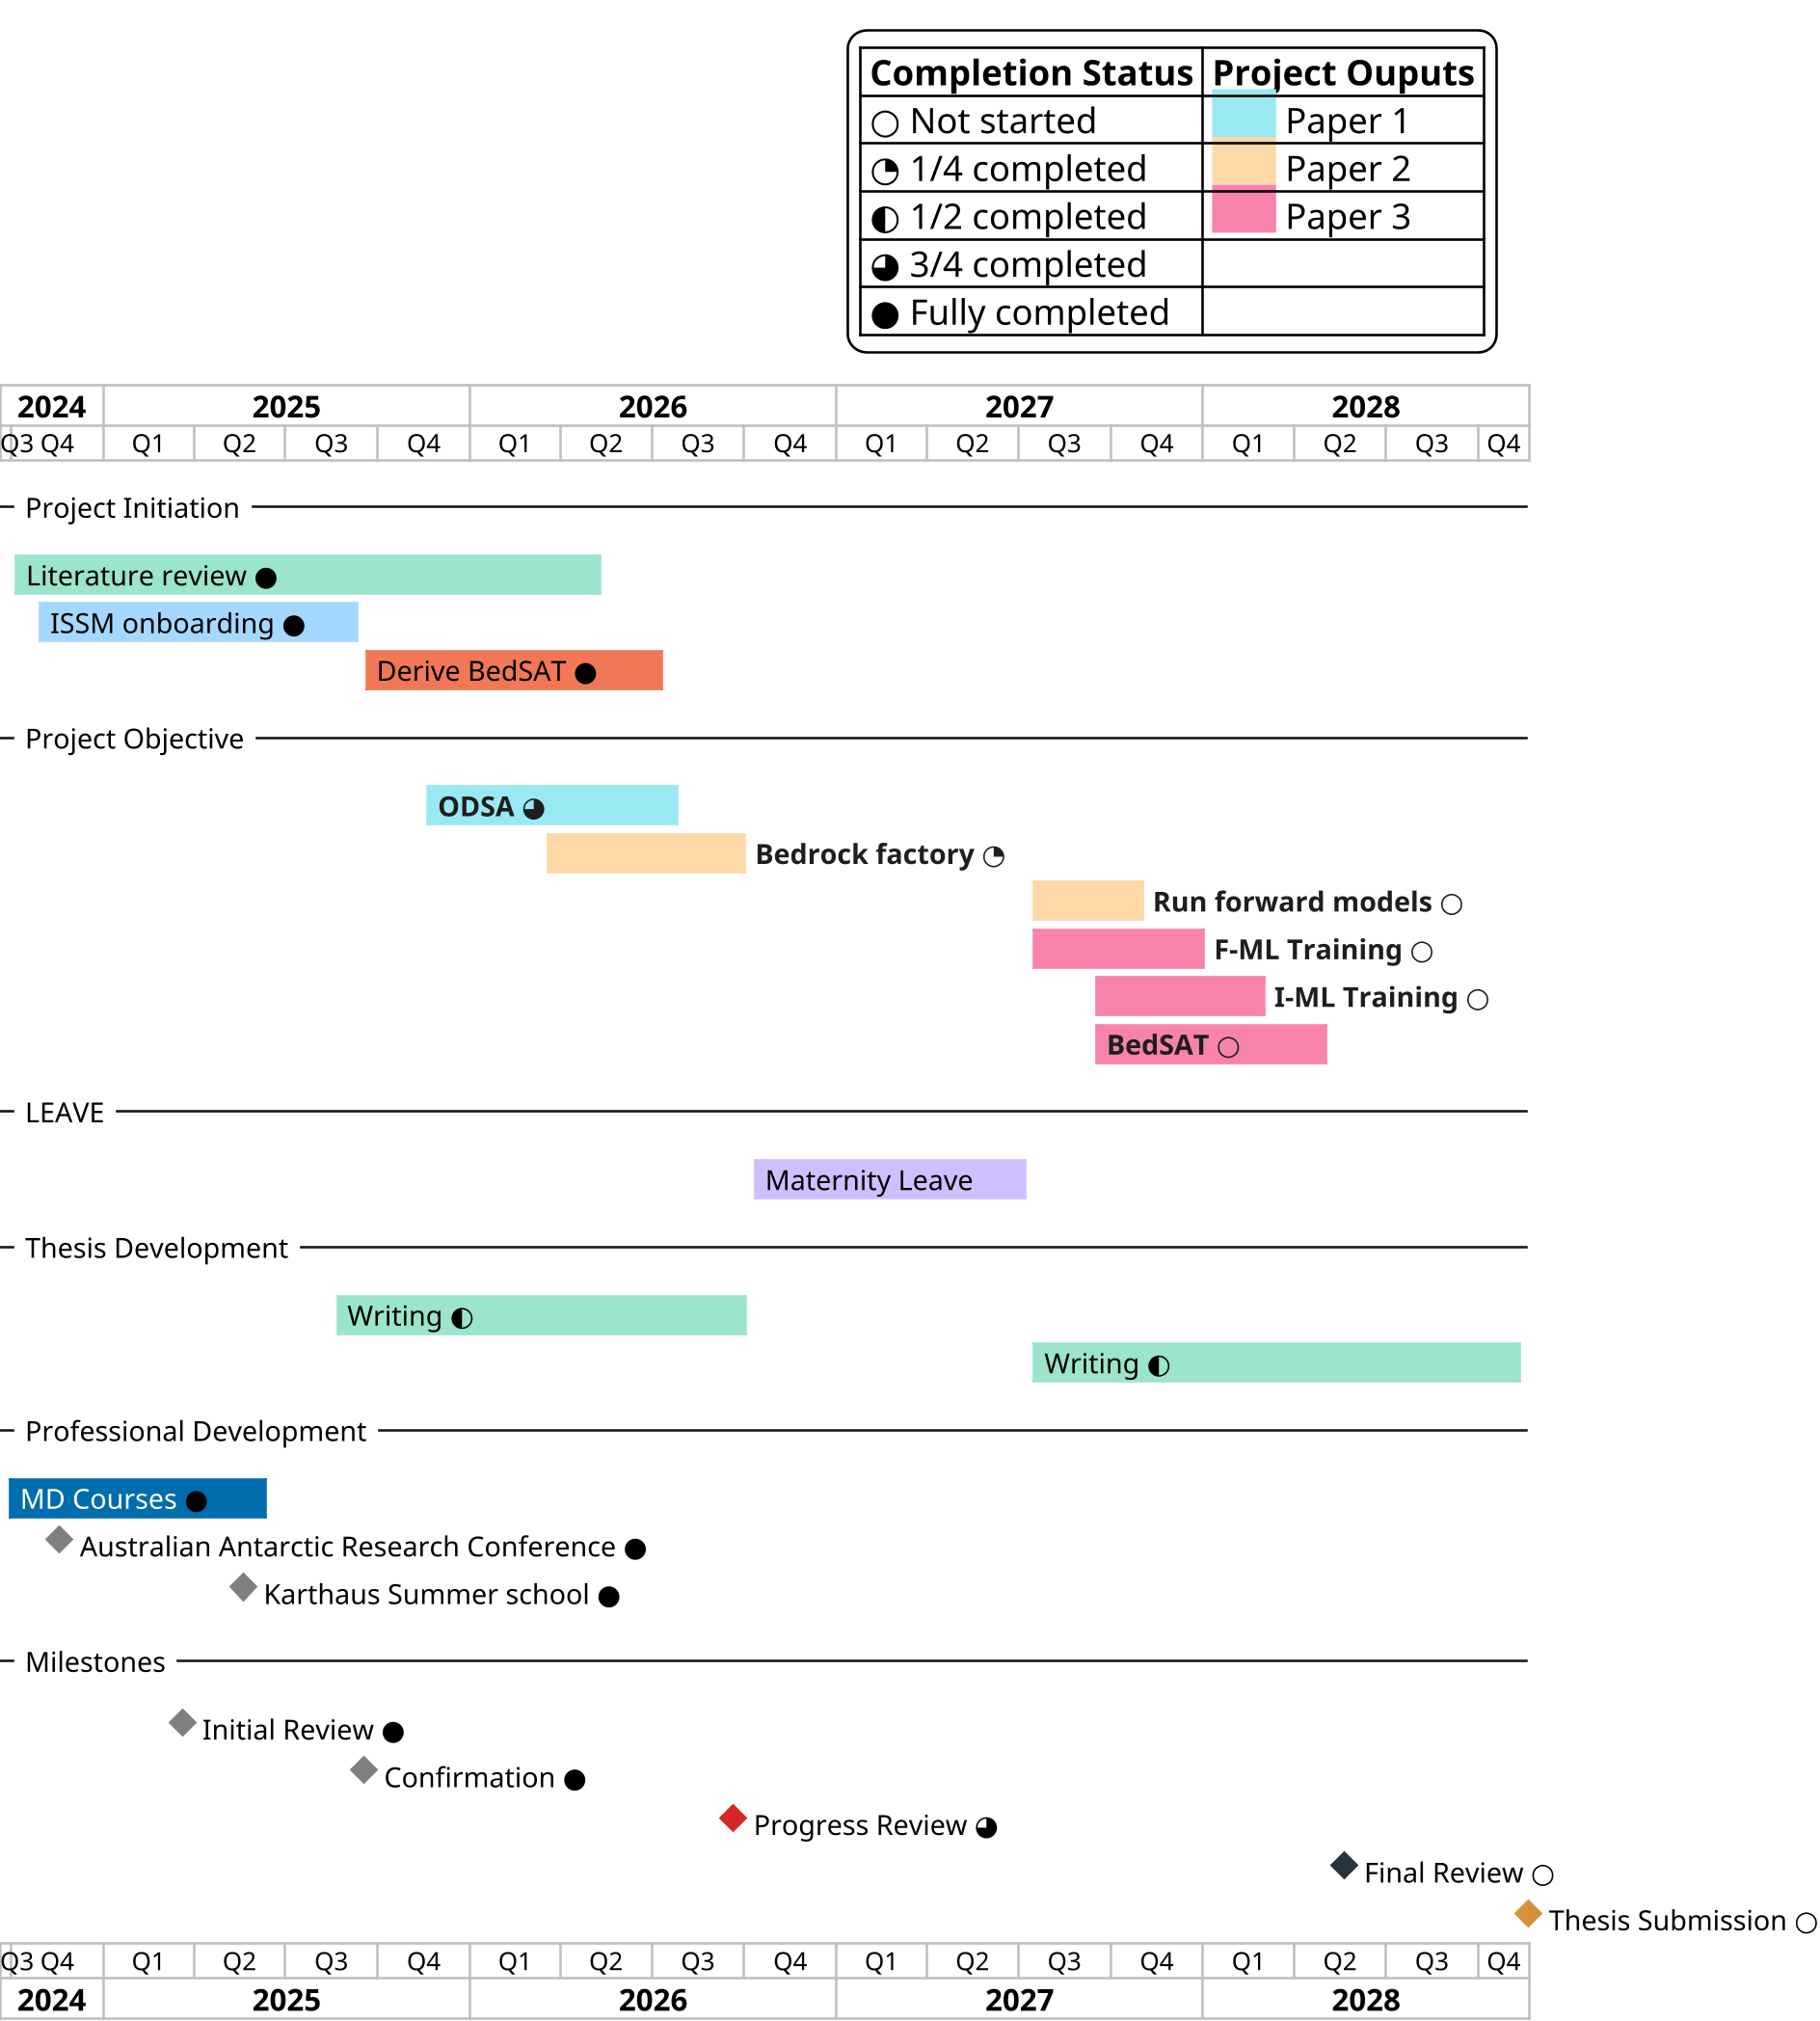
\includegraphics[width=1\linewidth]{figures/timeline.png}
\caption{Project timeline. In the Project Objective section, the
  colour of each bar shows which paper the task contributes to. The circle next to
  each item is an estimate of how complete it is: a quarter-filled circle means that the prototype of the code and workflow exists. A half-filled circle means that the task workflow is in progress. A three-quarter-filled circle means that the results are complete and a paper needs to be written up or the task needs to be officially approved by the panel. A filled circle means that the task is complete.}
\end{figure}